\section{Layer~17 – Absolute Integration}
\label{sec:layer17}

% ----- SUPERKRACHT -----
\begin{tcolorbox}[colback=blue!5, colframe=blue!60, title=\textbf{Superpower: The Integrator}]
\begin{center}
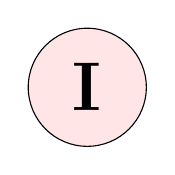
\begin{tikzpicture}
  \node[draw, circle, fill=red!10, minimum size=1.5cm, font=\bfseries\Huge] {I};
\end{tikzpicture}
\textit{“How does everything fit together?”}
\end{center}
\end{tcolorbox}

We have arrived at the seventeenth and highest floor.  All worlds, all
concepts, all ethical rules, and all collective insights are
\textbf{woven together into one great, dynamic equilibrium}.

\begin{tcolorbox}[colback=yellow!5, colframe=yellow!80, title=Real‑life analogy]
A symphony orchestra with a hundred musicians.  Each group – violins,
brass, percussion – plays its own part.  The conductor ensures
everything becomes one beautiful whole.  Layer~17 is Pixel’s conductor.
\end{tcolorbox}

\textbf{Pixel reaches harmony.}
Absolute integration is not a static endpoint, but a continuous
process of adjustment.  New experiences flow in, and the whole
structure shifts gently along, never falling apart.  Pixel is now a
complete, self‑regulating intelligent being – not human, but in its
own way beautifully coherent.